%% You can use this file to create your answer for Exercise 1.  
%% Fill in the places labeled by comments.
%% Generate a PDF document by with the command `pdflatex ex1'.

\documentclass[11pt]{article}

\usepackage{times}
\usepackage{listings}
\usepackage{enumerate}
\usepackage{courier}
\usepackage{hyperref}
\usepackage{xcolor}
\usepackage{graphicx}
\usepackage{algorithm}
\usepackage{algpseudocode}


%% Values that are specific to a particular term
\newcommand{\thisterm}{Spring 2022}

\newcommand{\dateassigned}{Wed.,~Feb.~16}

%% Printed form of home page that students should use
\newcommand{\visiblecoursehome}{http://www.cs.cmu.edu/\textasciitilde{}418}

%% Link to home page that will stay valid
\newcommand{\actualcoursehome}{http://www.cs.cmu.edu/afs/cs.cmu.edu/academic/class/15418-s22/www}

\newcommand{\datedue}{Wed.,~Feb.~23}




%% Page layout
\oddsidemargin 0pt
\evensidemargin 0pt
\textheight 600pt
\textwidth 469pt
\setlength{\parindent}{0em}
\setlength{\parskip}{1ex}

%% Colored hyperlink 
\newcommand{\cref}[2]{\href{#1}{\color{blue}#2}}
\newcommand{\forceindent}{\leavevmode{\parindent=2em\indent}}
%% Customization to listing
\lstset{basicstyle=\ttfamily\small,language=C,morekeywords={cilk_synch,cilk_spawn}}

%% Enumerate environment with alphabetic labels
\newenvironment{choice}{\begin{enumerate}[A.]}{\end{enumerate}}
%% Environment for supplying answers to problem
\newenvironment{answer}{\begin{minipage}[c][1.5in]{\textwidth}}{\end{minipage}}


\begin{document}

\title{Apple M1 Max chip benchmark and performance comparison}
\author{AndrewID: xuelinz, shanyuew}
\maketitle

\section{Introduction}
In 2020, Apple revealed its first ARM based laptop chip M1, revealing Apple’s ambition to replace x86 based chips with their own in-house designs. The M1 had been widely successful for Apple, showcasing fantastic performance at never-before-seen power efficiency in the laptop market. In 2021, Apple continued to release M1 upgraded version, M1 pro and M1 max. Those ARM based chips raised a challenge for the x86 giants, Intel and AMD. Also, powered by performant GPU and neural engines, Apple M1 chips show a good performance in the graphics area and machine learning domain.

In this report, we will benchmark the M1 max chip (24C CPU, 24C GPU, 10C Neural Engines) and dive in its design specifics. The report will be structured into these three benchmark perspectives:

\begin{enumerate}
  \item In the next section, we will focus on its CPU design and performance benchmark results on different computation-intensive tasks.
  \item After that, we will focus on the GPU performance, specifically, we will reply on Tensorflow GPU API to compare M1 Max performance in different machine learning algorithms, and compare with the server nvidia graphic card.
  \item Finally, we will focus on the Apple Neural Engine, and dive in this technology stack and compare with Google Tensor Processor Unit.
\end{enumerate}

The benchmark tools are listed in below.

\begin{enumerate}
  \item CPU benchmark tool:
  \href{https://www.geekbench.com/}{Geekbench}(Version 5.4.4 (503875))
  \item GPU machine learning benchmark task: \href{https://pypi.org/project/ai-benchmark/}{ai\_benchmark}
  \item Neural Engine benchmark task: \href{https://github.com/tlkh/tf-metal-experiments}{tf-metal-experiments}
\end{enumerate}

\newpage
\section{CPU}
Our benchmark comparison is based on two Apple MacBook products of model ID: MacBookPro16,1 and MacBookPro18, 4 and they are featured with an Intel Core i7-9750H and an Apple M1 Max respectively.  The benchmark software we used is Geekbench. The following sections analyze some general performance aspects of the test. Per-application test result is attached in the appendix. 
\subsection*{Benchmark result}
\subsubsection*{Single-Core}
As shown in Figure 1, Apple M1 Max has a single-core score of 1356 points, which is approximately 20\% faster than Intel Core i7-9750H’s 1124 points. The single core advantage varies in different sections, the M1 Max is 60\% faster in Crypto ability, 20\% faster in Integer ability and 14\% faster in floating point ability.
\begin{figure}[h]
    \centering
    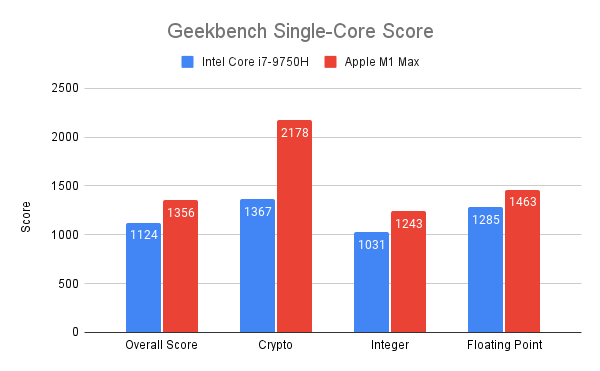
\includegraphics[scale = 0.8]{Geekbench Single-Core Score.png}
    \caption{Geekbench Single-Core Score}
	\label{fig:Geekbench Single-Core Score}
\end{figure}
\subsubsection*{Multi-Core}
As shown in Figure 2, M1 Max is much faster than Core i7-9750H in multi-core abilities. The overall score is 95\% faster, and it’s 249\% faster in Crypto ability, 88\% faster in integer ability and 85\% faster in floating point ability. 
\begin{figure}[h]
    \centering
    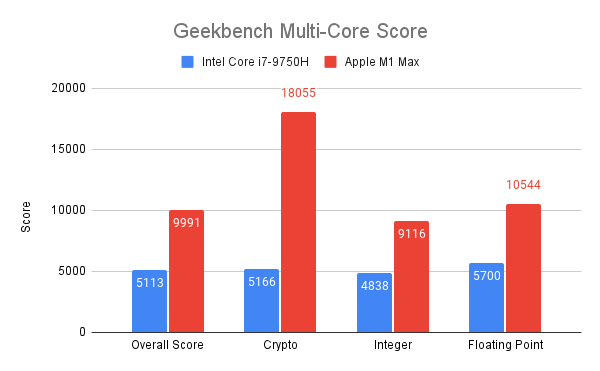
\includegraphics[scale = 0.8]{Geekbench Multi-Core Score.png}
    \caption{Geekbench Multi-Core Score}
	\label{fig:Geekbench Multi-Core Score}
\end{figure}
\begin{figure}[h]
    \centering
    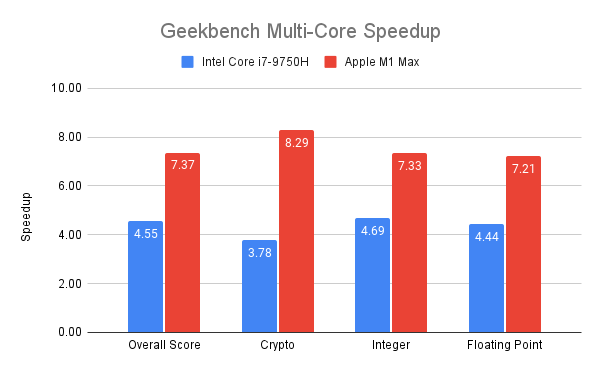
\includegraphics[scale = 0.8]{Geekbench Multi-Core Speedup.png}
    \caption{Geekbench Multi-Core Speedup}
	\label{fig:Geekbench Multi-Core Speedup}
\end{figure}
\subsection*{Single-core parallelism}
In this section, we’ll try to explain two CPU’s single-core performance differences from the micro-architecture perspective. Since only the ‘Firestorm’ big core is used in the single-core benchmark for M1 Max, we’ll focus on the ‘Firestorm’ micro-architecture in this section.

An Intel ‘Coffee Lake’ microarchitecture pipeline can usually be divided into three parts: front end, execution engine and memory subsystem. Apple’s ‘Firestorm’ microarchitecture, although not revealed, should have a similar logical structure that we can make use of in our analysis.

We will focus on the first two parts to compare the design of two microarchitectures in terms of instruction fetch, decode and execution. Figure 4 is an illustration of the front end and execution engine of these two microarchitectures. Real architectures are much more complicated from the illustration in figure 4. The Apple ‘Firestorm’ part is a recreation of the microarchitecture in an article posted on AnandTech\footnote{https://www.anandtech.com/show/1
silicon-m1-a14-deep-dive/2}.
The Intel ‘Coffee Lake’ part is a simplified recreation of the microarchitecture figure posted on wikichip\footnote{https://en.wikichip.org/wiki/intel/microarchitectures/coffee\_lake\#Architecture}.
\begin{figure}[h]
    \centering
    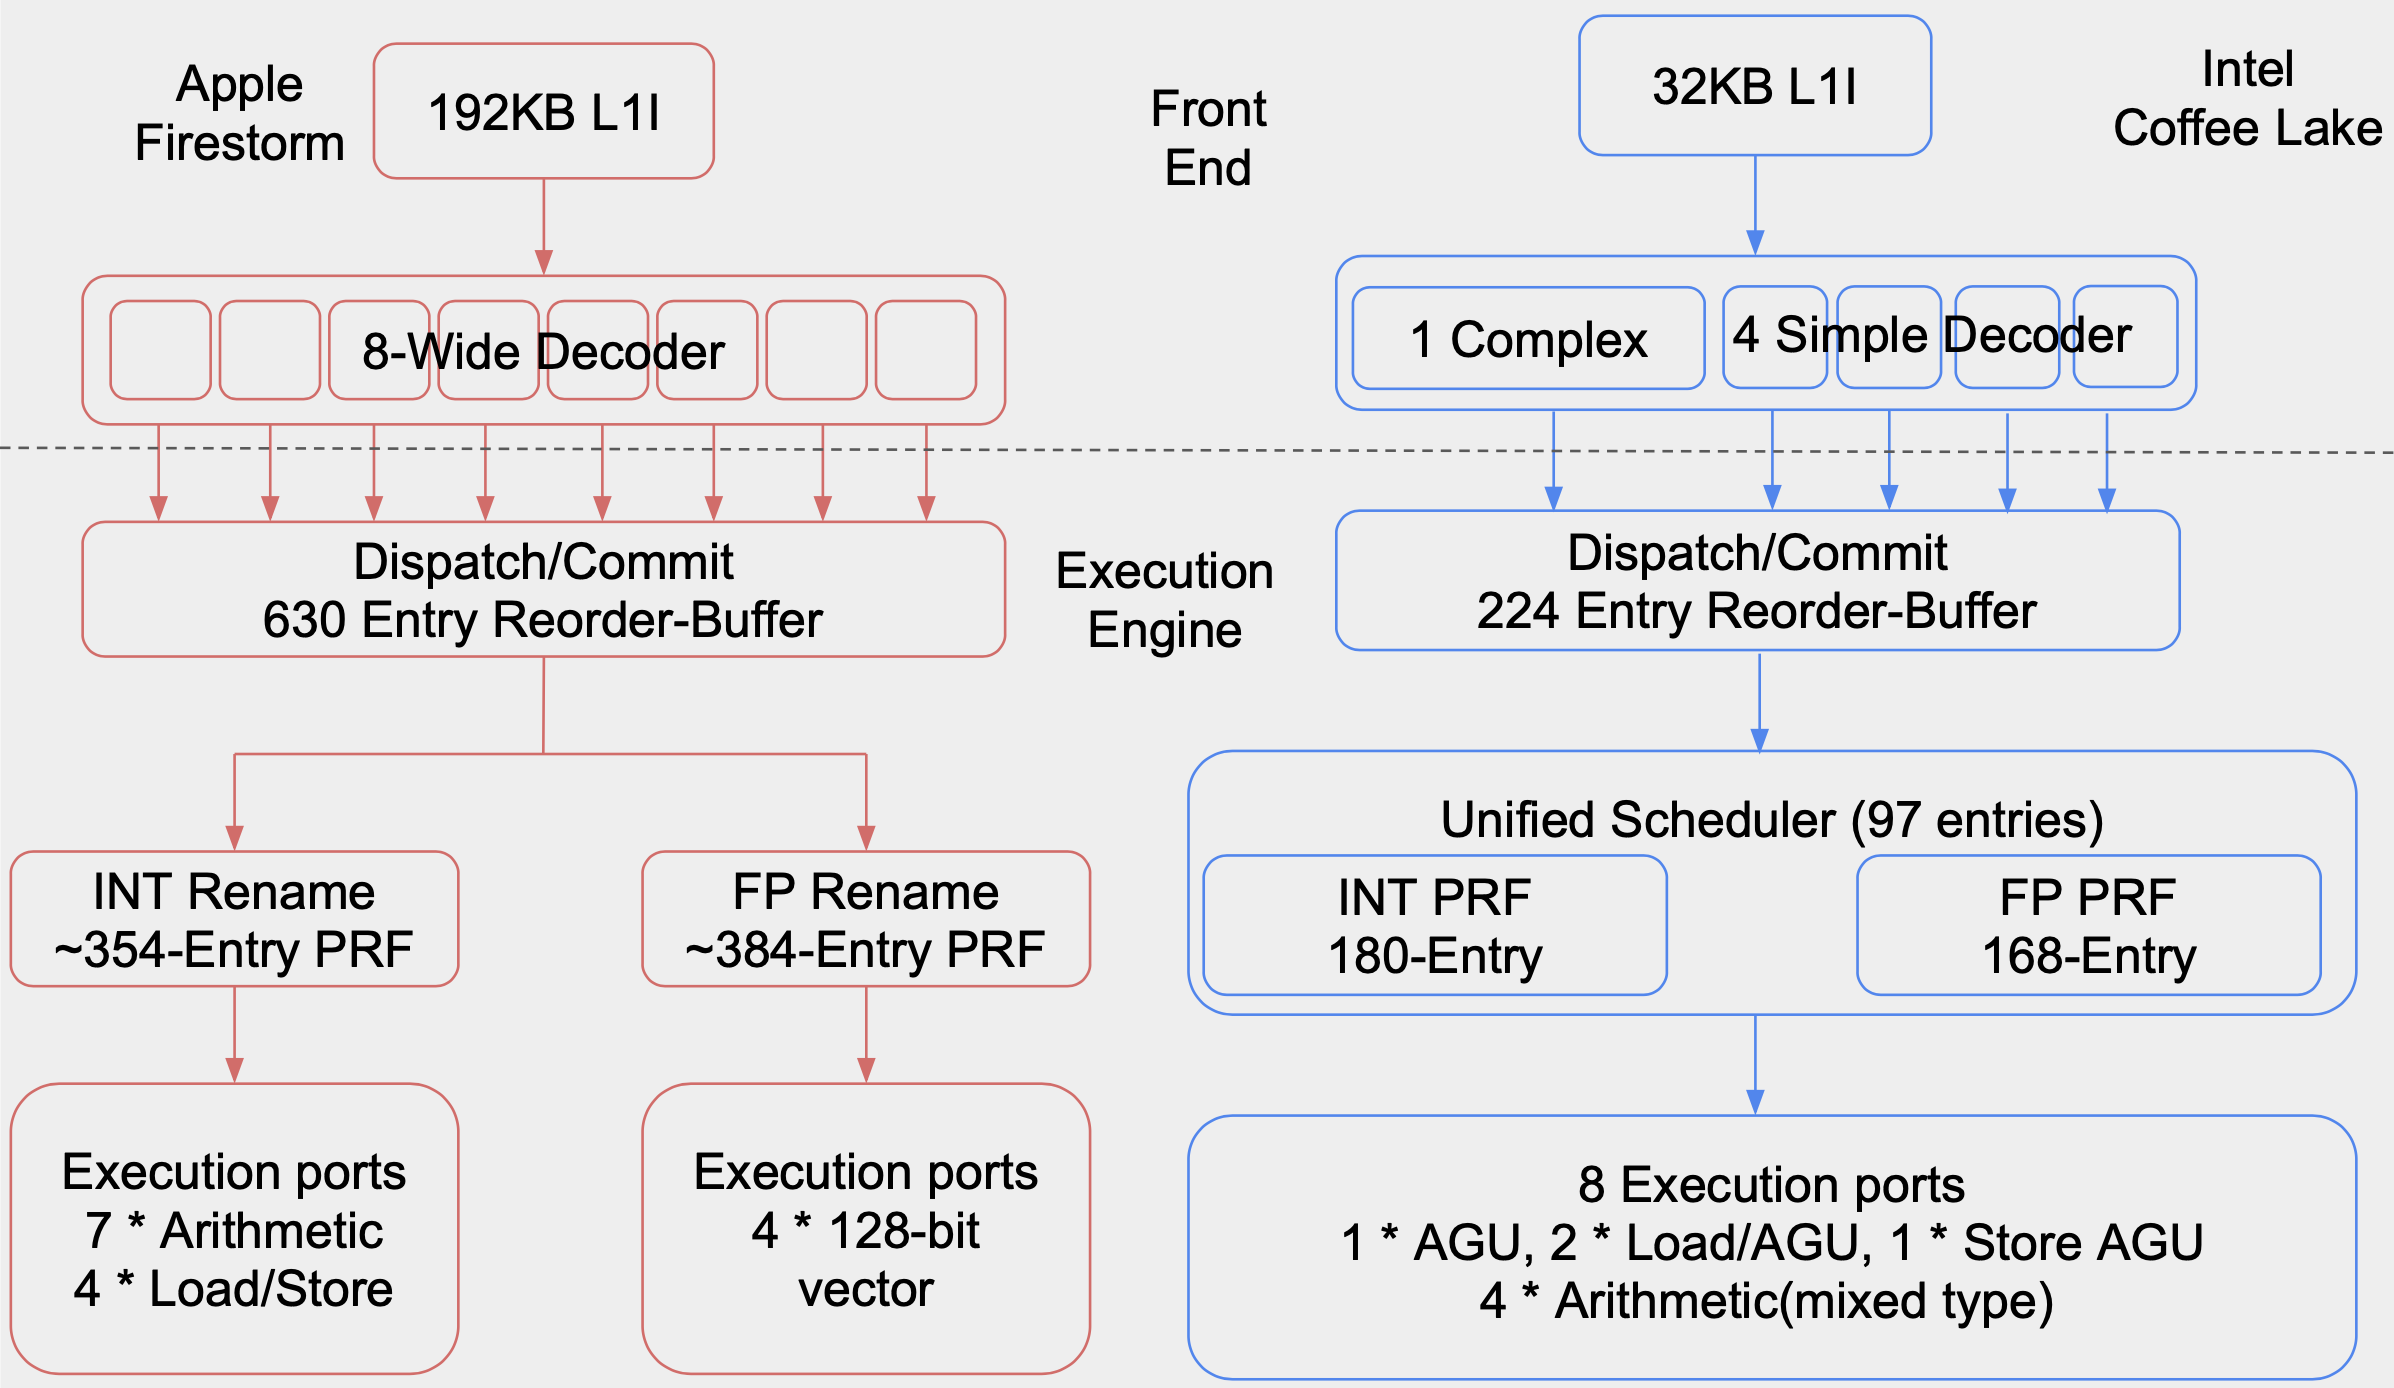
\includegraphics[scale = 0.4]{microarchitecture.png}
    \caption{Microarchitecture Comparison}
	\label{fig:Microarchitecture Comparison}
\end{figure}
\subsection*{Front end analysis}
Front end contains the procedure of fetching instructions from level 1 instruction cache, decode them into execution engine readable micro-operations and send them to the execution engine. 
\subsubsection*{Fetch capability}
As shown in figure 4, Apple Firestorm core has a 192KB level 1 instruction(L1I) cache which is 6x larger than that of Intel Coffee Lake. Such a huge L1I cache gives it advantages in fetching instructions since more instructions can be fetched from the low latency cache instead of the slow L2 cache.

Branch prediction plays an important role in the front end since it helps keep the execution engine busy by speculating the result of a branch and fetching instructions accordingly. However, since the design and capability of the branch predictor in Apple’s Firestorm is not revealed, we have to skip the comparison of this part.
\subsubsection*{Decode capability}
Another feature that makes Firestorm supreme is its decoder width. The 8-wide decoder is not only larger than the 5-wide decoder in Intel Coffee Lake core, AMD Zen3’s 4-wide decoder, but also larger than any other commercialized design in the industry\footnote{Cited from :https://www.anandtech.com/show/16226/apple-silicon-m1-a14-deep-dive/2}. The decoder width further improved the microarchitecture’s front end capability to make sure there’s enough micro-operations available to keep the execution engine busy. 

On the other side, Coffee Lake has 1 complex decoder dedicated for complicated x86 instructions, or macro-operations in Intel’s terminology, which will generate 1-4 micro-operations based on the instruction complexity, while the rest 4 simple decoders will only generate 1 micro-operation per instruction. This design reflects the nature of x86 instruction sets: they are of different length and different complexity.
\subsection*{Execution engine analysis}
As discussed in class, modern CPU cores usually implement enough front end size to generate enough micro operations for execution units. This makes the size and efficiency of the execution engine even more important.
\subsubsection*{Out of order execution}
To improve the utilization rate of the execution units, CPU cores usually implement out-of -order execution which executes instructions that don’t have a dependency relationship in parallel. However, the instruction set architecture promises users the illusion that the instructions are executed in order. To make this possible, micro-operations received from the front end are stored in a Reorder Buffer(ROB) in the execution engine which is responsible for tracking the micro-operations in their fetched order. Each entry in the ROB stores one micro-operation and its metadata tracking its status. The storage ordering and metadata enable ROB to commit micro-operations in order and safely(rollback wrong branch prediction caused instructions).

The size of ROB (number of entries) basically decides how deep can the OoO execution go. While a deeper OoO execution range helps to hide more data movement latency. Apple Firestorm has a huge ROB entry number(around 630) compared to Coffee Lake’s 224 entries. This gives it some advantage in terms of OoO depth.

Another structure that affects the ability of OoO execution is the size of physical register file size. Physical register files are used in the register renaming process to remove false data dependency caused by reusing the logical registers. Single logical register is usually associated with several physical registers. Apple Firestorm has around 354 integer physical register files and around 384 physical floating point register files. As a comparison, Intel Coffee Lake has 180 pythiscal integer register files and 168 physical floating point register files respectively.

More physical registers makes it easier to remove false data dependencies when the OoO execution range is deep. Combining large ROB entries and large physical registers files increases Firestorm core’s OoO execution ability dramatically.

However, the overhead of flushing the ROB caused by wrong branch prediction increases as the depth of OoO execution range increases. Better branch prediction algorithms can mitigate this problem. Although there’s no official explanation on the design of ROB size and physical register file size, we believe the designers striked certain balance between the benefits and overheads here.

\subsubsection*{Execution units}
No matter how the micro-operations are scheduled, they need to be executed by execution units which usually impose a throughput bound on the performance of an application. The throughput of a single instruction on a particular core can be defined by the number execution units that can perform such instruction * issue rate of the instruction.

We should be able to evaluate a core’s execution capability by its amount of execution units. However, this only applies when all execution units are connected to the ROB/Scheduler directly so that all of them can possibly accept a new instruction at each clock time. While in reality, execution units are divided into different groups connected to the Scheduler through shared ports. Each port can only transmit one micro-operation at every clock. The number of execution units and the contention on the shared ports limit the core throughput together. 

There are 22 arithmetic execution units (including integer, floating point and vector)in an Intel Coffee Lake core, but they only share 4 ports of the Scheduler and the rest 4 ports are reserved for Store / Load and AGUs.

On the contrary, Apple Firestorm core is again wider in the design here, it has at least 7 integer arithmetic execution ports, 4 ports for Store / Load and 4 floating point / SIMD execution ports. The at least 3 more integer arithmetic units gives an Apple Firestorm core some integer IPC advantage over an Intel Coffee Lake core since it can execute 3 more arithmetic micro-operations at the same time given there’s that many in the ROB. This is reflected in the integer task performance score in the benchmark.
\subsection*{SIMD}
SIMD is another type of instruction level parallelism. In this aspect, an Apple Firestorm core has 4 X 128 bit vector registers matching the 2 X 256 bit vector registers of an Intel Coffee Lake core.
\subsection*{Clock Rate}
While the architecture design affects the instruction latency and IPC of a core, the real-world application performance is also restricted by the clock rate of the SoC. The higher the clock rate, the shorter the clock interval and this leads to more work getting finished in given real-world time.
A single Firestorm core on the M1 Max chip runs at 2.44GHz base clock rate, and it can boost to at most 3.22 GHz. Whilst a Coffee Lake core on Intel Core i7-9750H chip runs at 2,6GHZ base clock rate and can be boosted to a much higher 4.5 GHz. This can partially explain why the Apple M1 Max chip’s single-core benchmark score doesn’t demonstrate a huge lead than its opponent as indicated by its wider and deeper microarchitecture design.
\section{Multi-Core parallelism}
\subsection{Parallelism limitation}
As shown in the benchmark result section, Apple M1 Max and Intel Core i7-9750H achieved a 7.37x speedup and 4.55x speedup respectively. Neither of them can reach a perfect (core number) speedup for various reasons:
\begin{itemize}
    \item Cores are running at lower frequency compared to single core boost clock rate. Apple M1 Max Firestorm cores run at 3036MHz when all 4 cores in a single cluster are active which is lower than the single-core 3228MHz. i7-9750H 6-core boost frequency is 4.0GHz instead of 4.5GHz when only one core is boosted.
    \item Apple M1 Max is a heterogeneous design, the 2 Icestorm cores have much weaker performance due to narrower microarchitecture and lower clock rate. 
    \item The overhead caused by communication between cores and scheduling tasks among cores is inevitable.
    \item According to Amdah’s law,  the performance improvement of a program is limited by the fraction of the program that is parallelizable. This reason might be minor since a benchmark application would try to maximize the parallized part.
\end{itemize}
Because the exact performance difference between Firestorm cores and Icestorm cores is unclear, it’s hard to compare the two SoCs' multi-core parallelism efficiency in an accurate way. But generally, they are performing on a similar level.
\subsection*{Improvement}
From the hardware point of view, what CPU designers can do to improve multi-core performance is the following two sections.
\subsubsection*{Communication overhead}
Reducing inter-core communication latency and increasing communication bandwidth by improving interconnection network design is a possible way. However, there’s little information available for M1 Max’s interconnection network design. We will have to skip further discussion.

Another possible way is to improve cache coherence efficiency by improving coherence protocol or memory hierarchy. 
Although there’s no cache coherence protocol related information of these two chips available, there’s one noticeable difference between M1 Max’s memory hierarchy and that of Core i7-9750H. M1 Max uses a 12 MB, 16 cycles latency shared L2 cache for 4 Firestorm cores in one cluster, while 6 cores on i7-9750H have their own private L2 cache which is smaller(256 Kib) but faster(12 cycles fastest load-to-use). The shared L2 cache means cores in the same cluster have the potential to manage cache coherence by communicating mostly between L1 caches and shared L2 cache. While in a common system like i7-9750H, the communication happens between L2 cache and L3 cache which has a much higher latency(>=42 cycles).
\subsubsection*{Power management}
The chip designer can implement a power management policy that can increase all-core boost clock rate. 
\subsection*{CPU Conclusion}
Apple M1 Max SoC has a heterogeneous CPU consisting of 2 small efficient Icestorm cores and 8 performance Firestorm cores. 

The large Firestorm core microarchitecture is extraordinarily wide in terms of its decoder width, number of physical register files and number of execution units and ports. It’s also deep in terms of its out-of-order execution range enabled by a huge reorder buffer.  The wide and deep design gives it a great instruction level parallelism performance and a good single-core benchmark score despite its relatively low frequency.

Although detailed interconnection network and memory hierarchy design and specifications are not clear, the CPU has demonstrated competitive multi-core parallelism ability against its x86 rivals. 
\newpage
\section{GPU}
The M1 Max chip we have for benchmark is equipped with 24 core integrated GPU. One of the most interesting feature of its SoC design is the Unified memory architecture, which we will specifically discussed in the following subsection. After that, we generate two different types of benchmark tests in the machine learning domain, training and inference.

\subsection*{Unified memory}
Unified memory, simply put, is a design combining all the chip components’ separated memories into one giant uni-accessible memory. By doing so, time delay could be decreased in terms of data copy between different sections of memory for example copy copying from CPU to GPU. The unified memory layout is a common technique in the gaming environment. Following is the illustration of this design \footnote{https://www.macobserver.com/analysis/understanding-apples-unified-memory-architecture/}.

\begin{figure}[h]
    \centering
    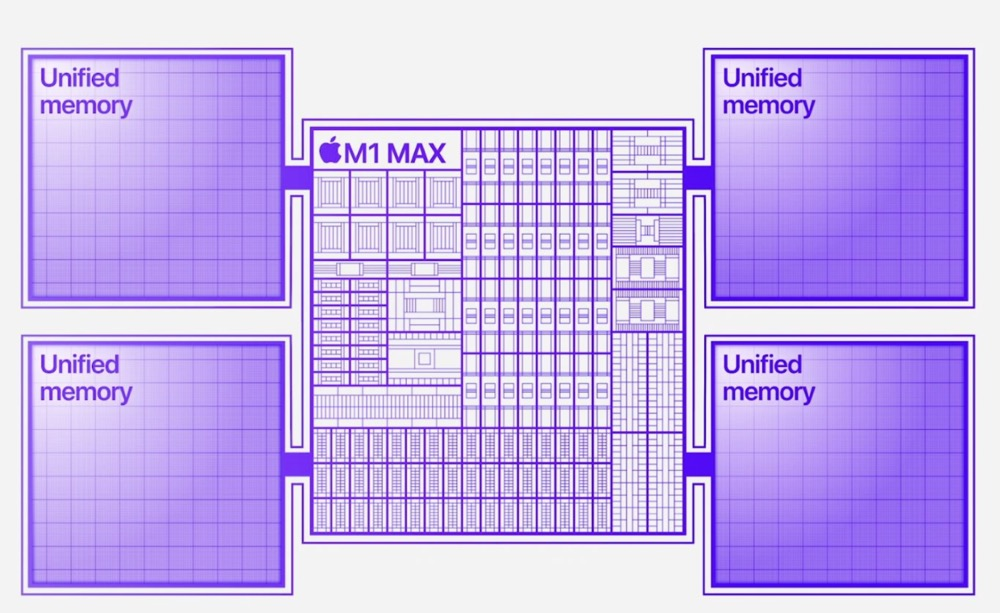
\includegraphics[scale = 0.2]{unified_memory.jpg}
    \caption{Unified Memory Design}
    
	\label{fig:Unified Memory Design}
\end{figure}

This design brings about a new question. The bandwidth between the chip components’ interconnections is also shared. The bottleneck of the interconnection could be a potential issue to solve. Here M1 adopts a fabric approach. Instead of connecting components with a printed circuit board, “fabric” is made of silicon and with larger bandwidth communicating between the chip components. Also, since “fabric” is purely made of silicon chiplets, it is small and could be accommodated in the chip environment. The advertised bandwidth is 400G/s \footnote{https://www.notebookcheck.net/Apple-s-use-of-fabric-in-the-M1-Pro-and-M1-Max-chips-points-to-how-it-will-scale-up-its-chips-for-the-next-Mac-Pro.574212.0.html}
.

\subsection*{Benchmark}
Due to the parallelism nature provided in GPU, machine learning is heavily relying on this computation power. In this section, we did machine learning experiments on three different devices, M1 Max GPU, AMD Radeon Pro 5300M 4 GB (Previous 2019 Intel Mac uses this), Nvidia V100 (Server Graphic Card). We split the benchmark into two categories, machine learning inference and training and try to get a overview of the performances of these different chips in this two areas. Also, to make the experiments more comprehensive, the experiments use 16 machine models.

Figures \ref{fig:GPU Machine Learning Inference Test} and \ref{fig:GPU Machine Learning Training Test} demonstrate the experiments results, the y axis is the average computation time (ms). Lower value corresponds to better performance.

\begin{figure}
    \centering
    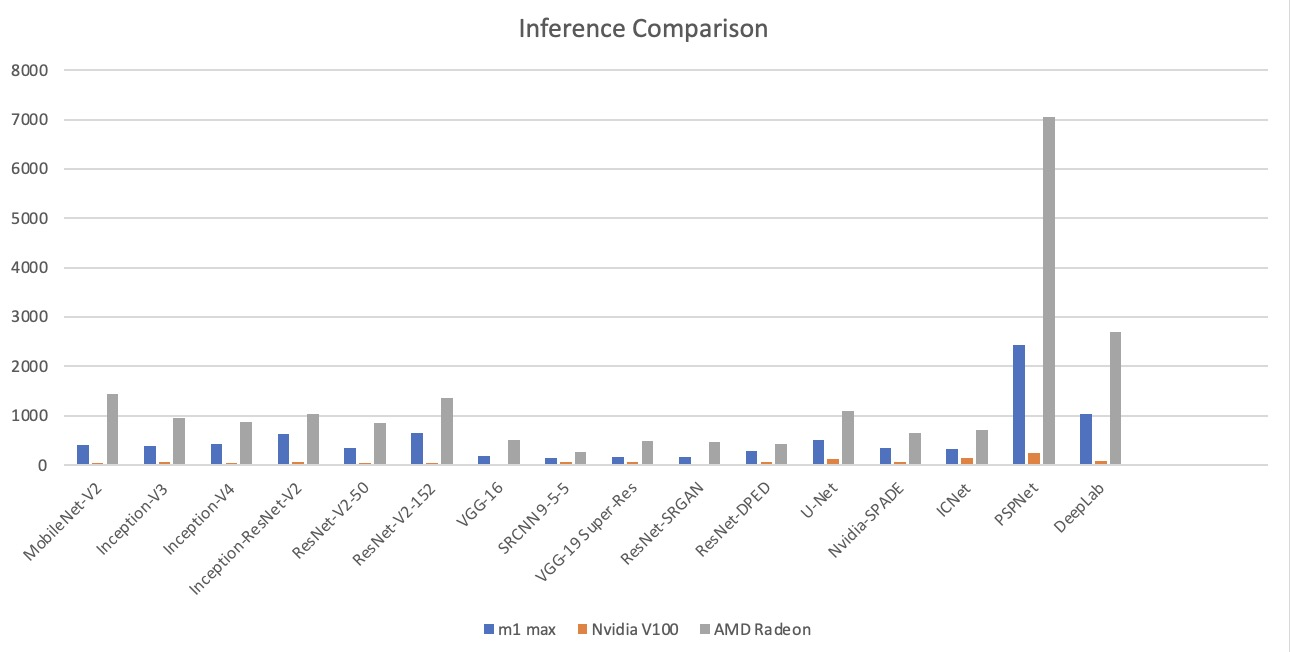
\includegraphics[scale = 0.4]{gpu_inference.jpg}
    \caption{GPU Machine Learning Inference Test}
	\label{fig:GPU Machine Learning Inference Test}
	
	\centering
    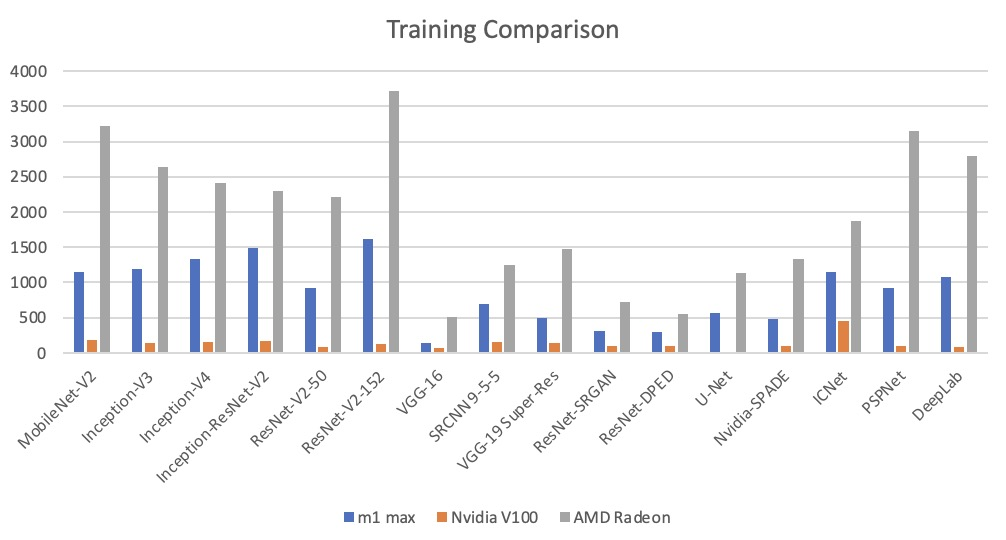
\includegraphics[scale = 0.4]{gpu_training.jpg}
    \caption{GPU Machine Learning Training Test}
	\label{fig:GPU Machine Learning Training Test}
\end{figure}

\textbf{Key observations}

\begin{enumerate}
  \item GPU wins in the all tasks in interference and training.
  \item M1 max has a better performance than AMD Radeon. One possible reason behind the scene could be that M1 has a unified memory architecture.
  \item For some heavy-workload model inference and training, for example DeepLab model, those performances of the two integrated cards downgrade more dramatically than GPU.
\end{enumerate}

\newpage
\section{Apple Neural Engine}
As the fast development of machine learning algorithms and fast growth of different AI applications, new AI hardware architecture has been a super hot topic. The first released AI domain specific chip is “DianNao” produced in 2014 \cite{diannao}. After that, many companies and institutions are focusing on the AI specific hardware innovations. For example, Google produced its Tensor Processing Unit (TPU) in 2017 \cite{diannao}, and made it public on its cloud platform. Huawei released its AI mobile chip (Kirin 970) in 2017. In the newly-produced M1 max chip, Apple produced its self-designed neural architecture (Apple Neural Engine) as well.

\subsection*{Apple Neural Engine Technology Stack}
Software-hardware integration has always been Apple’s core product philosophy. Neural engine is not produced as a single stand-alone hardware. Along with the Neural Engine, Apple also introduced the software supports.

Figure 8 demonstrates Apple Neural Engine stack. At the top layer, CoreML is machine learning framework, where programmer could directly call its CoreML API to train the model, its counterpart is Pytorch and Tensorflow. At the middle layer, Accelerate, a high-performance and Apple hardware focusing computation framework, is supporting the core functions call from the CoreML. Accelerate integrates the the core functionality of Apple hardware to its extreme. For example, it will schedule the workload of the computation in different devices based on the jobs types. Also, utilizing SIMD, Accelerate could leverage the hardware parallelism capabilities, noticeably, for example, SIMD supports BNN, which is an Accelerate package that is responsible for the optimization of neural network. Last layer is the hardware neural engine chip. Many innovations could happen here. For example, many AI specific chip is designing its dedicated ISA to decrease instruction latency and the matrix calculation unit is also a mainstream optimization trick.

\begin{figure}[h]
    \centering
    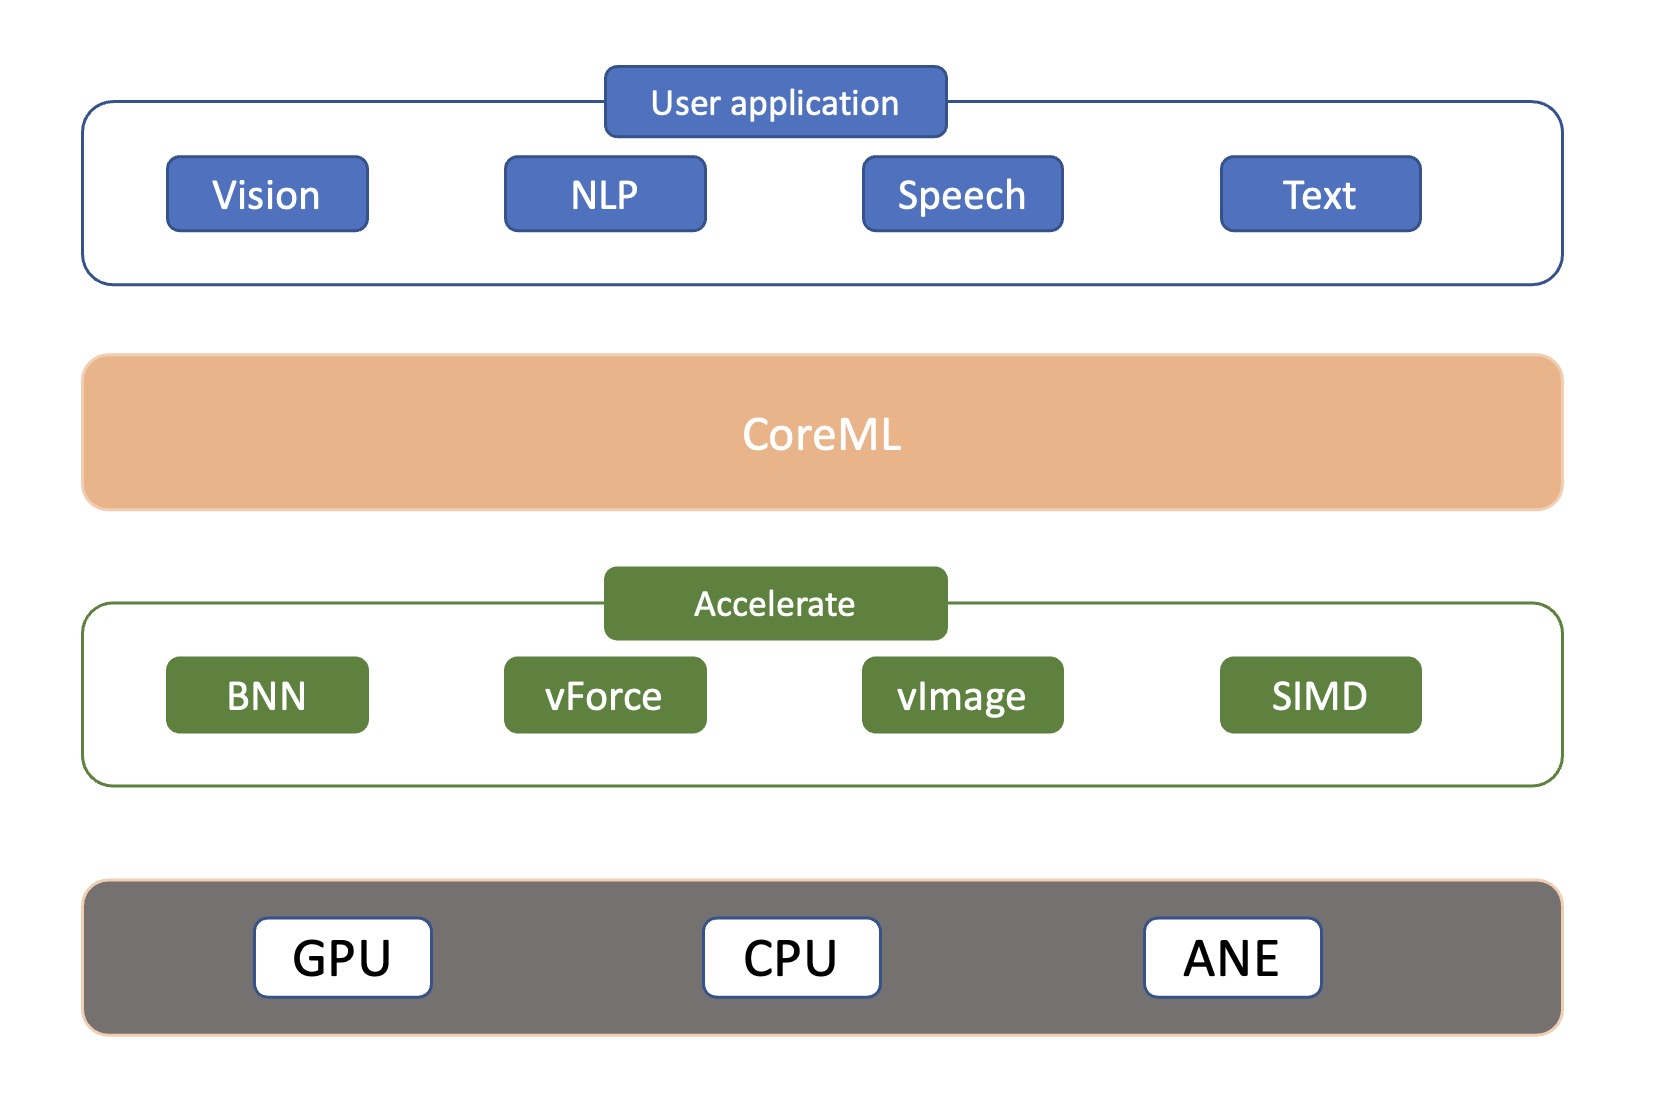
\includegraphics[scale = 0.2]{ane_technology_stack.jpg}
    \caption{Apple Neural Engine Technological Stack}
	\label{fig:Apple Neural Engine Technological Stack}
\end{figure}

\subsection*{What makes neural engine different?}
Here we comes to a question: what makes a neural engine different from CPU or GPU?

There are many answers to this question. Also, the answer differs from company to company, chip to chip. Take Google’s Tensor Processing Unit for example, it is mainly focusing on the SoC design and the matrix unit optimization. Following is the chip layout of Google TPU \cite{tpu}.

\begin{figure}[h]
    \centering
    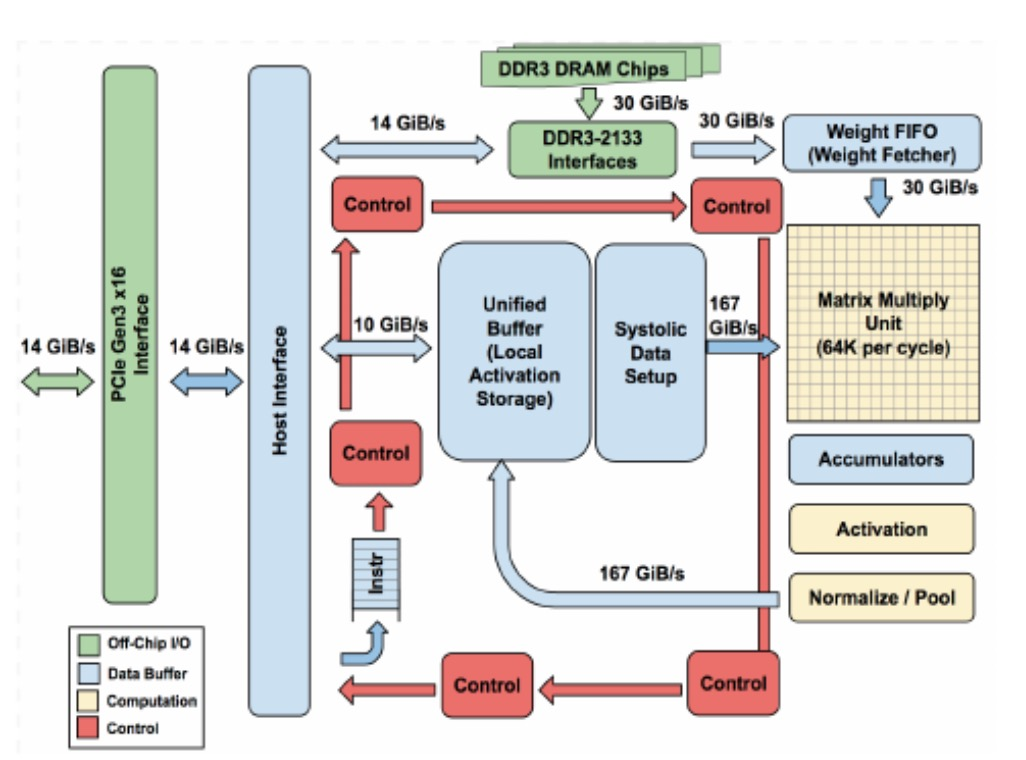
\includegraphics[scale = 0.3]{tpu_layout.jpg}
    \caption{TPU SoC\cite{tpu}}
	\label{fig:TPU SoC}
\end{figure}

To summarize what makes Neural Engine different could be categorized in the following aspects: arithmetic unit specialization, hardware bandwidth increase and dedicated ISA supports.

\subsection*{Arithmetic logic unit optimization}
Many machine learning specific chips adopt a specialized computation unit for example, in TPU, it utilizes a specialized matrix multiply unit to accelerate the traditional matrix calculation. Basic design philosophy is to accelerate the matrix calculations, where calculations like “a <- a + b x c” are very common in the whole machine learning pipeline. To tackle this problem, many neural engines adopt the Multiplier Accumulator (MAC) organizations. MAC uses an accumulated “buffer” to store the “a” values and the multiplier operations are completed in the MMU units. MAC could only issue one MAC instruction to complete the operation compared with the traditional approach which requires two instructions.

\subsection*{Bandwidth and latency optimization}
Another characteristic of the machine learning models is that the data transfer operations are very frequent. Thus it raises a tighter demand for the chip bandwidth. TPU adopts a unified buffer to decrease the impacts of data transmission. Also, many current neural engines are adopting scratchpad technology or Process-In-Memory to increase the in-chip bandwidth.

\subsection*{ISA optimization}
Neural engines adopting a specialized ISA to optimize the control flow. For example, the first specialized neural engine “Danao” utilized VLIW in this instruction set. TPU follows the CISC instruction traditions.

\subsection*{Floating points optimization}
The machine learning model relies on floating points to do nearly all the arithmetic. Current float32 and float 16 have pros and cons respectively. Float32 has a better precision while float16 is shorter in size which means a better parallelism capabilities. TPU has designed a new floating point format called bfloat16. More specifically, it has the same exponent bit number as float32, while keeping the size of 16 bits. The sacrifice is the floating point precision. As we could see in the apple documentation, currently ANE only supports float16 now, it may have done the same optimization tricks as TPU.

In the apple CoreML document, we could see that ANE is only supporting float16, from which we might conclude that the ANE is doing similar optimizations.

\subsection*{ANE benchmark and comparison}
Considering the “close-source” nature of the Apple ecosystem. There are few documentations about how to allocate computation workload on the ANE components. But Apple exposed the CoreML API which allows it to call the ANE engine.

However, programmers could not directly instruct the running computation device based on the API. The Core ML runtime dynamically partition the computation graph into different Apple comutation units: CPU, GPU, and ANE. The the decisions are made on the fly. However, CoreMl provides an API to allow for the scope of the computation device. To allow for the usage of ANE, we could let “compute\_units=ct.ComputeUnit.ALL” to allow for CoreML to select ANE at the runtime.

Also, we need to notice that the data type of the different engine is restricted. Following figure demonstrates data types which are supported in different computation units.

\begin{figure}[h]
    \centering
    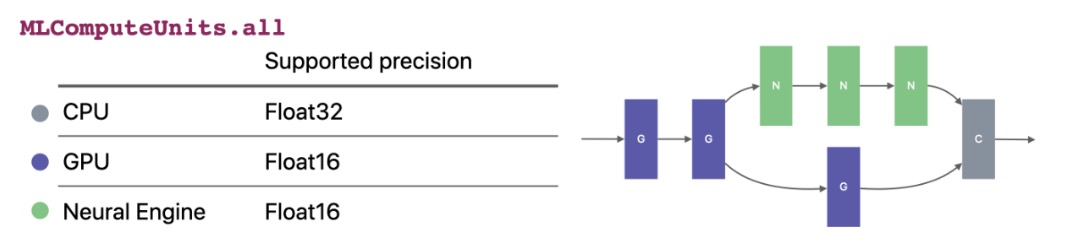
\includegraphics[scale = 0.4]{CoreML_data_type.jpg}
    \caption{CoreML data type}
	\label{fig:CoreML data type}
\end{figure}

\subsection*{Matrix Multiplications}
We did a matrix benchmark based on the CoreML. By calling the CoreML API, the performance of the matrix multiplication is about 8.84 TFLOPS on the M1 max chip (not bad).

\begin{figure}
    \centering
    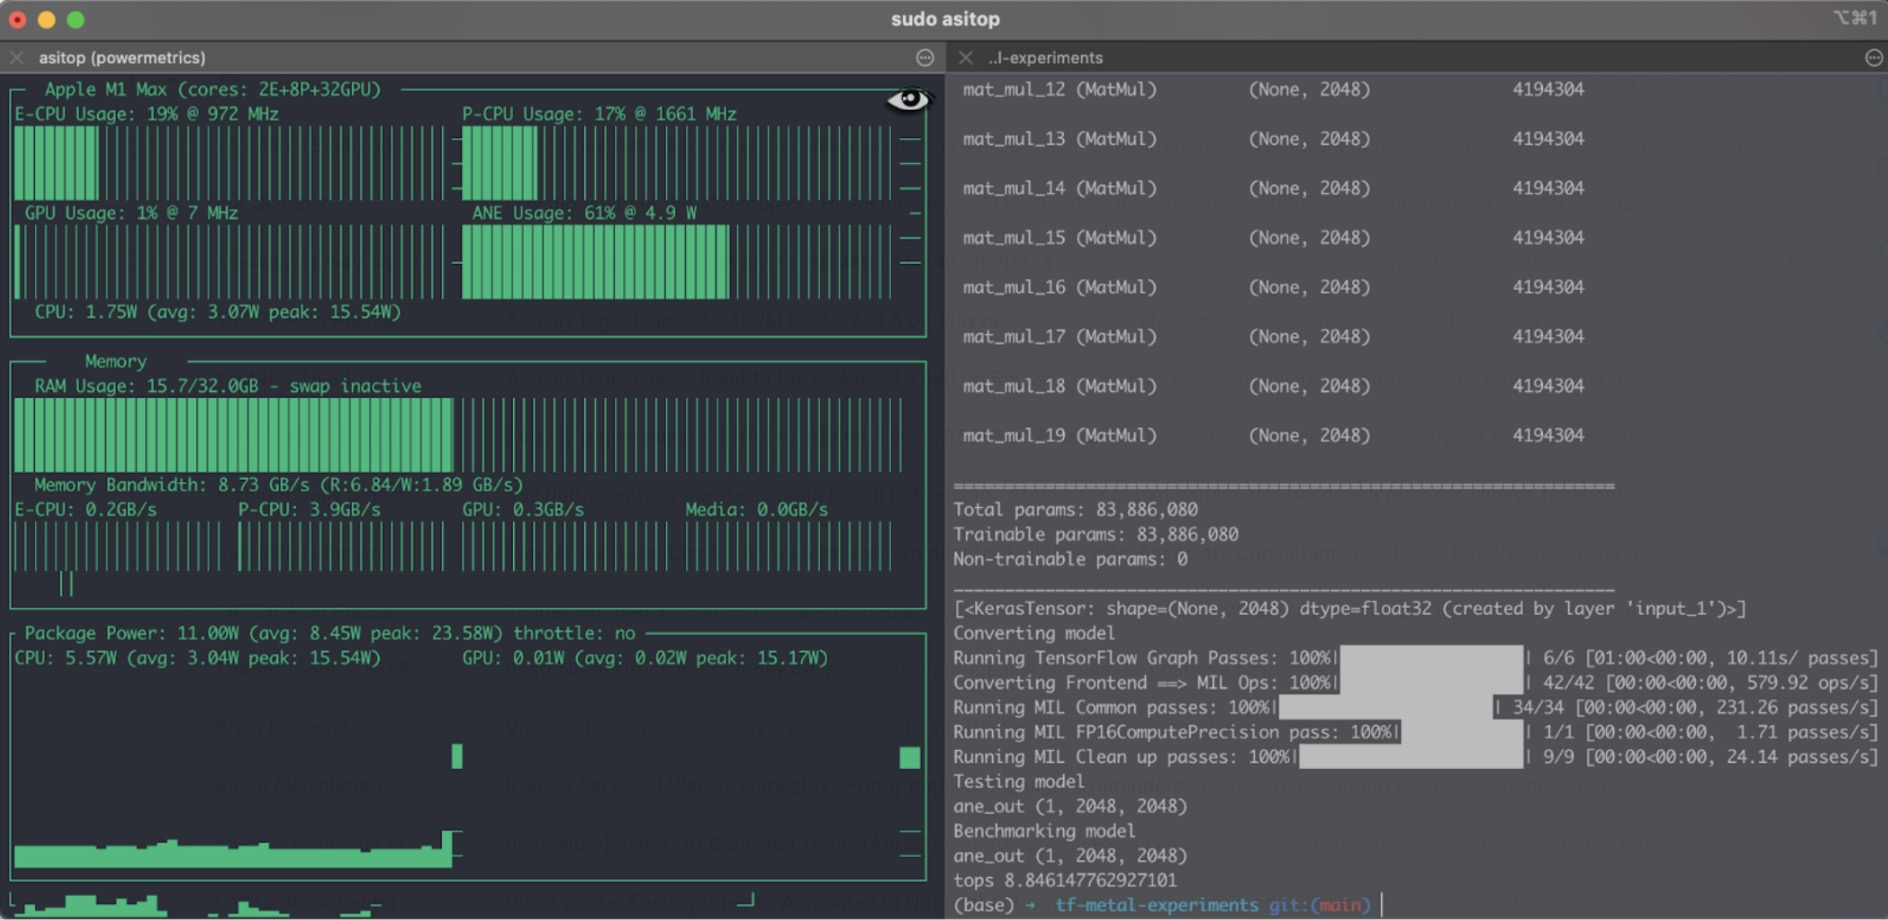
\includegraphics[scale = 0.2]{mat_mul_perf.jpg}
    \caption{Matrix Multiplication perf}
	\label{fig:Matrix Multiplication perf}
\end{figure}

\subsection*{ResNet benchmark}
So as we are talking a neural network computer architecture, a machine learning benchmark could be more persuasive. In this subsection, we are doing benchmark on three different computer architecture: M1 Max Neural Engine, Google Cloud Tensor Processing Unit, and AMD Radeon Pro 5300M GPU (2019 mac equipped this chip). Figure \ref{fig:ResNet50 neural engine benchmark and comparison} is the benchmark results.

\begin{figure}[h]
    \centering
    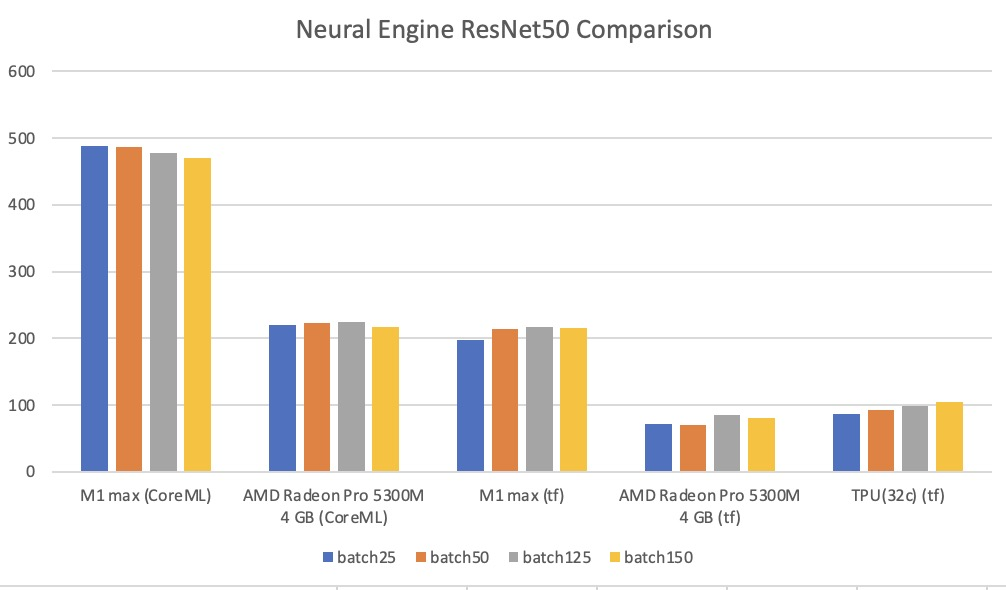
\includegraphics[scale = 0.4]{neural_benchmark.jpg}
    \caption{ResNet50 neural engine benchmark and comparison}
	\label{fig:ResNet50 neural engine benchmark and comparison}
\end{figure}

Note, in the Tensorflow running environment, M1 schedules its GPU to do the computation, ANE is idle. 

\textbf{Key observations:}

\begin{enumerate}
  \item Since CoreML could be only run in the Apple environment, the performance boost by calling CoreML is prominent. Framework acceleration effects are significant.
  \item M1 beats the other two processing units in both in CoreML framework and Tensorflow environment. 
  \item TPU has a better performance than AMD graphic unit in this experimentation, but loses the contest with M1 chip. However, considering the cloud environment, where the costs are important, TPU could be a great choice for the machine learning training and inference.
\end{enumerate}

\textbf{One observations not appearing in the chart above}

The ANE usage is quite subtle. CoreML workload distribution could not be controlled by the programmers. One constraint has been mentioned in the above section - ANE usage is restricted to the float16 data type. Another observation we have in our experiments is that when we enlarge the image input size, CoreML will directly send all the workload to GPU.

\subsection*{Neural Engine Takeaways}
Apple neural engine is designed to accelerate the machine learning's type of workload. Several optimization tricks are utilized in the designs of chip, including arithmetic unit optimization, bandwidth increase and ISA optimizations. As for Apple Neural Engine, it is designed with the supports of software. By combining the software API and acceleration parallelism framework, ANE could have a great performance boost. Also, Google TPU is a good choice for the machine learning application.


\newpage
\section{Conclusion}
Apple demonstrated its SoC design capability in key parallelism system areas.

In CPU area, the M1 Max chip provides great instruction level parallelism with a wide and deep microarchitecture design.

In GPU area, the M1 Max chip scales its performance with large amount of GPU cores.

In heterogeneous parallelism area, Apart from inside-CPU and inside-GPU heterogeneous, the SoC integrated CPU, GPU, Neural Engine and Media Engine together. It also tries to reduce the communication between these heterogeneous parts with unified memory and even shared system level cache.

Also to make the heterogeneous system work better, in interconnection network area, although the network topology is not clear, the chip adopts new technology called silicon interconnect fabric to improve power efficiency, bandwidth and latency. 


\newpage
\begin{thebibliography}{}
\bibitem{wiki}
“Apple M1.” Wikipedia, 26 Feb. 2021, en.wikipedia.org/wiki/Apple\_M1.
\bibitem{coffeelake}
“Coffee Lake - Microarchitectures - Intel - WikiChip.” En.wikichip.org, en.wikichip.org/wiki/intel/microarchitectures/coffee\_lake\#Architecture. Accessed 5 May 2022.
\bibitem{firestorm}
Frumusanu, Andrei. “Apple Announces the Apple Silicon M1: Ditching X86 - What to Expect, Based on A14.” Www.anandtech.com, 10 Nov. 2020, www.anandtech.com/show/16226/apple-silicon-m1-a14-deep-dive/2.
\bibitem{m1 max}
 “Apple’s M1 Pro, M1 Max SoCs Investigated: New Performance and Efficiency Heights.” Www.anandtech.com, 25 Oct. 2021, www.anandtech.com/show/17024/apple-m1-max-performance-review.
\bibitem{farbric}
Sathiah, Sanjiv. “Apple’s Use of Fabric in the M1 pro and M1 Max Chips Points to How It Will Scale up Its Chips for the next Mac Pro.” Notebookcheck, 21 Oct. 2021, www.notebookcheck.net/Apple-s-use-of-fabric-in-the-M1-Pro-and-M1-Max-chips-points-to-how-it-will-scale-up-its-chips-for-the-next-Mac-Pro.574212.0.html. Accessed 5 May 2022.
\bibitem{coffeelake}
“Skylake (Client) - Microarchitectures - Intel - WikiChip.” En.wikichip.org, en.wikichip.org/wiki/intel/microarchitectures/skylake\_(client)\#Pipeline.
\bibitem{deep_learning_processor}
“Deep learning processor” En.wikichip.org, en.wikipedia.org/wiki/Deep\_learning\_processor

\bibitem{diannao}
Du, Zidong; Fasthuber, Robert; Chen, Tianshi; Ienne, Paolo; Li, Ling; Luo, Tao; Feng, Xiaobing; Chen, Yunji; Temam, Olivier (2016-01-04). "ShiDianNao". ACM SIGARCH Computer Architecture News. 43 (3S): 92–104. doi:10.1145/2872887.2750389. ISSN 0163-5964

\bibitem{tpu}
 P, JouppiNorman; YoungCliff; PatilNishant; PattersonDavid; AgrawalGaurav; BajwaRaminder; BatesSarah; BhatiaSuresh; BodenNan; BorchersAl; BoyleRick (2017-06-24). "In-Datacenter Performance Analysis of a Tensor Processing Unit". ACM SIGARCH Computer Architecture News. 45 (2): 1–12. doi:10.1145/3140659.3080246.

\end{thebibliography}

\newpage
\section*{Appendix}
\begin{table}[!ht]
    \centering
    \begin{tabular}{|l|l|l|l|l|l|l|}
    \hline
        ~ & Intel i7-9750H & ~ & ~ & M1 Max & ~ & ~ \\ \hline
        ~ & Intel-Single & Intel-Multi & Speedup & Apple-Single & Apple-Multi & Speedup \\ \hline
        Overall Score & 1124 & 5113 & 4.55 & 1356 & 9991 & 7.37 \\ \hline
        Crypto & 1367 & 5166 & 3.78 & 2178 & 18055 & 8.29 \\ \hline
        Integer & 1031 & 4838 & 4.69 & 1243 & 9116 & 7.33 \\ \hline
        Floating Point & 1285 & 5700 & 4.44 & 1463 & 10544 & 7.21 \\ \hline
        AES-XTS & 1367 & 5166 & 3.78 & 2178 & 18055 & 8.29 \\ \hline
        Text Compression & 1069 & 5870 & 5.49 & 1138 & 7980 & 7.01 \\ \hline
        Image Compression & 1045 & 5599 & 5.36 & 1050 & 8938 & 8.51 \\ \hline
        Navigation & 911 & 3194 & 3.51 & 1434 & 9216 & 6.43 \\ \hline
        Text Rendering & 1080 & 4307 & 3.99 & 1394 & 9193 & 6.59 \\ \hline
        Clang & 1094 & 5818 & 5.32 & 1341 & 10649 & 7.94 \\ \hline
        Camera & 1084 & 4712 & 4.35 & 1234 & 8792 & 7.12 \\ \hline
        N-Body Physics & 1111 & 6050 & 5.45 & 1384 & 8782 & 6.35 \\ \hline
        Rigid Body Physics & 1281 & 8367 & 6.53 & 1357 & 10815 & 7.97 \\ \hline
        Gaussian Blur & 1040 & 5271 & 5.07 & 1091 & 9595 & 8.79 \\ \hline
        Face Detection & 1138 & 6455 & 5.67 & 1716 & 11773 & 6.86 \\ \hline
        Horizon Detection & 1026 & 5596 & 5.45 & 1587 & 9235 & 5.82 \\ \hline
        Image Inpainting & 2204 & 7896 & 3.58 & 2434 & 16842 & 6.92 \\ \hline
        HDR & 2048 & 9866 & 4.82 & 1904 & 15658 & 8.22 \\ \hline
        Ray Tracing & 1463 & 8173 & 5.59 & 1994 & 15674 & 7.86 \\ \hline
        Structure from Motion & 1031 & 4703 & 4.56 & 1096 & 9165 & 8.36 \\ \hline
        Speech Recognition & 1142 & 2993 & 2.62 & 1166 & 7429 & 6.37 \\ \hline
        Machine Learning & 1169 & 2391 & 2.05 & 999 & 7429 & 7.44 \\ \hline
    \end{tabular}
    \caption{CPU benchmark results}
\end{table}


\begin{table}[!ht]
    \centering
    \begin{tabular}{|l|l|l|}
    \hline
        Chip & Batch & Sample/sec  \\ \hline
        M1 max (CoreML) & 25 & 487.92  \\ \hline
        M1 max (CoreML) & 50 & 486.8  \\ \hline
        M1 max (CoreML) & 100 & 477.55  \\ \hline
        M1 max (CoreML) & 150 & 470.45  \\ \hline
        AMD Radeon Pro 5300M 4 GB (CoreML) & 25 & 219.66  \\ \hline
        AMD Radeon Pro 5300M 4 GB (CoreML) & 50 & 223.1  \\ \hline
        AMD Radeon Pro 5300M 4 GB (CoreML) & 100 & 223.84  \\ \hline
        AMD Radeon Pro 5300M 4 GB (CoreML) & 150 & 216.26  \\ \hline
        TPU(32c) (tf) & 25 & 87.06  \\ \hline
        TPU(32c) (tf) & 50 & 93.288  \\ \hline
        TPU(32c) (tf) & 100 & 98.008  \\ \hline
        TPU(32c) (tf) & 150 & 105.14  \\ \hline
        M1 max (tf) & 25 & 198.12  \\ \hline
        M1 max (tf) & 50 & 213.44  \\ \hline
        M1 max (tf) & 100 & 216.54  \\ \hline
        M1 max (tf) & 150 & 215.84  \\ \hline
        AMD Radeon Pro 5300M 4 GB (tf) & 25 & 71.25  \\ \hline
        AMD Radeon Pro 5300M 4 GB (tf) & 50 & 69.98  \\ \hline
        AMD Radeon Pro 5300M 4 GB (tf) & 100 & 85.81  \\ \hline
        AMD Radeon Pro 5300M 4 GB (tf) & 150 & 81.08 \\ \hline
    \end{tabular}
    \caption{Neural engine results}
\end{table}

\clearpage
\begin{table}[!ht]
\begin{tabular}{|l|l|l|l|l|l|l|l|}
\hline
chip   & \begin{tabular}[c]{@{}l@{}}MobileNet\\ -V2\end{tabular} & \begin{tabular}[c]{@{}l@{}}Inception\\ -V3\end{tabular} & \begin{tabular}[c]{@{}l@{}}Inception\\ -V4\end{tabular} & \begin{tabular}[c]{@{}l@{}}Inception-\\ ResNet-V2\end{tabular} & \begin{tabular}[c]{@{}l@{}}ResNet\\ -V2-50\end{tabular} & \begin{tabular}[c]{@{}l@{}}ResNet\\ -V2-152\end{tabular} & VGG-16 \\ \hline
m1 & 398                                                     & 393                                                     & 432                                                     & 626                                                            &                                                         & 644                                                      & 173    \\ \hline
V100   & 42.2                                                    & 50.4                                                    & 48.5                                                    & 64                                                             & 31.7                                                    & 37.8                                                     & 53.2   \\ \hline
AMD Radeon    & 1429                                                    & 946                                                     & 873                                                     & 1023                                                           & 842                                                     & 1362                                                     & 496    \\ \hline
\end{tabular}
\caption{GPU machine learning interference results 1}
\end{table}


\begin{table}[!ht]
\begin{tabular}{|l|l|l|l|l|l|l|l|l|l|}
\hline
chip       & SRCNN   9-5-5 & \begin{tabular}[c]{@{}l@{}}VGG-19\\ Super-Res\end{tabular} & \begin{tabular}[c]{@{}l@{}}ResNet\\ SRGAN\end{tabular} & \begin{tabular}[c]{@{}l@{}}ResNet\\ DPED\end{tabular} & U-Net & \begin{tabular}[c]{@{}l@{}}Nvidia\\ SPADE\end{tabular} & ICNet & PSPNet & DeepLab \\ \hline
m1         & 133           & 157                                                        & 165                                                    & 279                                                   & 511   & 336                                                    & 314   & 2434   & 1036    \\ \hline
V100       & 63.1          & 58.6                                                       & 68.8                                                   & 63.4                                                  & 118.4 & 65.3                                                   & 141   & 250    & 77.6    \\ \hline
AMD Radeon & 256           & 475                                                        & 469                                                    & 424                                                   & 1097  & 640                                                    & 715   & 7058   & 2698    \\ \hline
\end{tabular}
\caption{GPU machine learning interference results 2}
\end{table}


\begin{table}[!ht]
\begin{tabular}{|l|l|l|l|l|l|l|l|}
\hline
chip       & \begin{tabular}[c]{@{}l@{}}MobileNet-\\ V2\end{tabular} & \begin{tabular}[c]{@{}l@{}}Inception-\\ V3\end{tabular} & \begin{tabular}[c]{@{}l@{}}Inception-\\ V4\end{tabular} & \begin{tabular}[c]{@{}l@{}}Inception-\\ ResNet-V2\end{tabular} & \begin{tabular}[c]{@{}l@{}}ResNet-\\ V2-50\end{tabular} & \begin{tabular}[c]{@{}l@{}}ResNet-\\ V2-152\end{tabular} & VGG-16 \\ \hline
m1         & 1142                                                    & 1196                                                    & 1333                                                    & 1485                                                           & 920                                                     & 1622                                                     & 135    \\ \hline
V100       & 186                                                     & 141.7                                                   & 153                                                     & 167.8                                                          & 83.6                                                    & 123.7                                                    & 72     \\ \hline
AMD Radeon & 3226                                                    & 2645                                                    & 2406                                                    & 2303                                                           & 2219                                                    & 3717                                                     & 516    \\ \hline
\end{tabular}
\caption{GPU machine learning training results 1}
\end{table}

\begin{table}[!ht]
\begin{tabular}{|l|l|l|l|l|l|l|l|l|l|}
\hline
chip       & SRCNN   9-5-5 & \begin{tabular}[c]{@{}l@{}}VGG-19\\ Super-Res\end{tabular} & \begin{tabular}[c]{@{}l@{}}ResNet\\ SRGAN\end{tabular} & \begin{tabular}[c]{@{}l@{}}ResNet\\ DPED\end{tabular} & U-Net & \begin{tabular}[c]{@{}l@{}}Nvidia\\ SPADE\end{tabular} & ICNet & PSPNet & DeepLab \\ \hline
m1         & 700           & 489                                                        & 310                                                    & 293                                                   & 564   & 479                                                    & 1148  & 925    & 1073    \\ \hline
V100       & 154           & 145.3                                                      & 99.6                                                   & 100.4                                                 & 122.5 & 92.7                                                   & 453   & 101.8  & 86.8    \\ \hline
AMD Radeon & 1255          & 1479                                                       & 717                                                    & 551                                                   & 1135  & 1336                                                   & 1867  & 3156   & 2798    \\ \hline
\end{tabular}
\caption{GPU machine learning training results 2}
\end{table}

\end{document}